
\title{Correttore BERT}
\author{
        Sebastiano Caccaro
}


\documentclass[12pt]{article}
\usepackage[utf8]{inputenc}
\usepackage{amssymb}
\usepackage{amsmath}
\usepackage[italian]{babel}
\usepackage{hyperref}
\usepackage{color,soul}
\usepackage{float}
\usepackage{listings}
\usepackage{tikz}
\usetikzlibrary{positioning}


\lstset{  
  xleftmargin=0.05\textwidth, xrightmargin=.2\textwidth,
}

\begin{document}
\maketitle
\newcommand{\E}{È}


\abstract{In questo documento è descritto il correttore sviluppato sulla base di un modello BERT}


\section{BERT}
\textbf{BERT}\cite{bert} (Bidirectional Encoder Representations from Transformers) è una tecnica di machine learing basata sui transformer utilizzata nel campo del NLP (Natural Language Processing) per il pre-training di modelli linguistici.


%TODO ESPANDERE https://en.wikipedia.org/wiki/BERT_(language_model)
%TODO Riferimenti bibliografici anche al paper originale di BERT

\subsection{Modello}
Allenare da zero un modello è un processo altamente dispendioso. Per la nostra applicazione è stato quindi deciso di utilizzare un modello pre-allenato su dei corpora in lingua italiana, chiamato \textit{dbmdz/bert-base-italian-xxl-uncased}\cite{bert_it}.
%TODO Posso espadnere citando i corpus su quale questo modello è stato allenato.

\subsection{Libreria}
La libreria Transformers\cite{transformers} fornisce una API unificata per utilizzare diverse architetture di transformer, fra le quali anche BERT.	\\
La libreria mette a disposizione una serie di task. In particolare, per la nostra applicazione, verrà utilizzato "Fill Mask".\\
\label{sec:fillmask}
Per utilizzare questa funzione, è innanzitutto necessario mascherare una parola all'interno di un frase. Per fare ciò, basta sostituire \textit{"[MASK]"} alla parola scelta. Dando questa frase in input al sistema, verranno generate della parole candidate al posto della maschera, insieme alla probabilità che ogni parola sia quella corretta. Ognuna delle parole generate è scelta in base al contesto della frase.\\
\E\ inoltre importante sottolineare come per una frase non sia possibile mascherare più di una parola.\\
Ad esempio, partendo dalla frase
\begin{center}
\textit{"Roma è la capitale d'Italia."}
\end{center}
è possibile mascherare \textit{"capitale"} e ottenere la seguente frase:
\begin{center}
\textit{"Roma è la [MASK] d'Italia."}
\end{center}
Il sistema genera quindi dei candidati per sostituire la maschera:
\begin{enumerate}
\item \textit{"capitale"} con probabilità 0.906
\item \textit{"città"} con probabilità 0.030
\item \textit{"storia"} con probabilità 0.009
\item \textit{"regina"} con probabilità 0.005
\item \textit{"culla"} con probabilità 0.005
\end{enumerate}
\E\ chiaro come in questo caso l'opzione 1 sia quella corretta.

\section{Sistema di correzione}
\subsection{Funzionamento generale}
Data una qualsiasi frase contenente degli errori in input, lo scopo del sistema di correzione è quello di fornire in output la stessa frase senza gli errori. A tale scopo è necessario:
\begin{itemize}
\item Individuare gli errori
\item Correggere gli errori individuati
\item Non introdurre nuovi errori
\end{itemize}
Il sistema di correzione è organizzato come una pipeline, la quale può essere composta da più moduli. Ogni modulo può essere ripetuto una o più volte. Concettualmente, ogni modulo è modellato per individuare e correggere uno specifico tipo di errore.\\
Più formalmente un modulo può essere definito come la seguente funzione:
\begin{equation}
M: T \mapsto T\prime
\end{equation}
dove $T$ e $T\prime$ sono rispettivamente la stringa di testo originale e quella corretta.\\
\E\ quindi possibile definire una pipeline di correzione come segue:
\begin{equation}
P: f_1 \circ f_2 \circ ... \circ f_n
\end{equation}
dove ogni $f_i$ è un modulo.

\subsection{Modulo di Correzione Token}
Il modulo di correzione token individua e corregge in ogni frase gli errori a livello di parola. Sono considerati errori solamente i cosiddetti non-word errors, ovvero quelle parole che non sono presenti nel vocabolario utilizzato per la correzione.\\
%TODO Potrei dire che il modulo può lasciare delle frasi inalterate
Il modulo agisce nelle seguenti fasi:
\begin{enumerate}
\item Tokenizzazione
\item Individuazione degli errori
\item Correzione degli errori
\item Detokenizzazione
\end{enumerate}

\subsubsection{Tokenizzazione}
In questa fase lo scopo è quello di dividere una frase nelle parole che la compongono, ad esempio:
\begin{center}
\textit{"I seminaristi hanno bisogno dell'attenzione personale"}
\end{center}
diventa:
\begin{center}
\textit{"I", "seminaristi", "hanno", "bisogno", "dell", "'", "attenzione", "personale"}
\end{center}
Per svolgere questo task è utilizzata la libreria python NLTK\cite{nltk} (The Natural Language Toolkit), che mette a disposizione una funzione apposita. L'output di questa funzione è inoltre ulteriormente processato per evitare che il carattere "'" (apostrofo singolo) venga considerato come parte di un token. \E\ infatti fondamentale per le fasi successive che i simboli di punteggiatura siano separati dalle parole vere e proprie.
%TODO fare esempi di scomposzione
%TODO Possibile notazione

\subsubsection{Individuazione degli errori}
In questa fase lo scopo è quello di individuare i token contenti degli errori, che verranno poi sottoposti a correzione.\\
Dato un dizionario di parole, un token viene considerato errato se non è presente all'interno del dizionario. Sono però definite delle eccezioni a questa regola:
\begin{itemize}
\item Tutti i token di un carattere sono considerati corretti. Questo approccio permette di evitare di provare a correggere parole frammentate o segni di punteggiatura non presenti nel vocabolario.
\item Se un token non è presente nel vocabolario ed è seguito da un token di apostrofo, è probabile che sia avvenuta l'elisione di una vocale. In questo caso, vengono generate cinque versioni diverse della stessa parola, ognuna terminante con una vocale diversa. Se almeno una di queste è presente nel dizionario, il token è considerato corretto.\\
Nell'esempio proposto in precedenza si nota la sequenza \textit{"dell", "'", "attenzione"}. Il token \textit{"dell"} potrebbe non essere presente nel dizionario. Si verifica quindi se almeno uno fra \textit{"della","delle","delli","dello","dellu"} è presente nel dizionario. In questo caso, quindi, il token \textit{"dell"} è considerato corretto.
\end{itemize}

\subsubsection{Correzione degli errori}
Una volta che una parola viene segnala come errata è necessario tentare di correggerla. Il processo ha inizio detokenizzando, ovvero ricomponendo, la frase originaria. Nel farlo, si sostituisce \textit{"[MASK]"} al token errato.\\
La detokenizzazione è implementata a partire dal modulo \textit{TreebankWordDetokenizer} della libreria NLTK. L'output di questo modulo viene successivamente ulteriormente processato per rimuovere caratteristiche indesiderate, come degli spazi prima di alcuni segni di punteggiatura.\\
A questo punto, il sistema descritto nella \autoref{sec:fillmask} genera i possibili token candidati. Il candidato scelto è quello che minimizza la distanza di Levenshtein fra sé stesso e il token errato: non viene fatto uso della probabilità prodotta dal sistema.\\
Può accadere che anche il migliore dei candidati prodotti possa non rappresentare una correzione plausibile. Ciò si verifica quando la distanza di Levenshtein fra il token errato e il candidato supera una certa soglia. In questi casi è preferibile non correggere l'errore.

\subsubsection{Detokenizzazione}
A questo punto, se uno o più token all'interno della frase sono stati corretti, la frase viene detokenizzata e restituita. Altrimenti, viene restituita la frase originale.

\subsection{Modulo di Correzione Split}
Il modulo di correzione di split serve a correggere tutti quelli errori che risultano nella frammentazione di una o più parole adiacenti. Un esempio di tale tipo di errore è la frase:
\begin{center}
\textit{"coinvolsero ogni uomo e ogni donna, procurando."}
\end{center}
che diventa
\begin{center}
\textit{"coinvolsero ogni uomo e o g n i donna, p r o c u r a n d o."}
\end{center}
\E\ chiaro da questo esempio come le parole \textit{ogni} e \textit{procurando} siano state frammentate.\\
Il funzionamento del modulo può essere diviso nelle seguenti fasi:
\begin{itemize}
\item Individuazione degli errori
\item Correzione degli errori
\end{itemize}

\subsubsection{Individuazione degli errori}
Gli errori di frammentazione vengono individuati dalla seguente espressione regolare:

\begin{lstlisting}[language=Python]
r'(?:\s|^)(\w(?:\W?\s\w{1,2}){3,})(?:\W|\s|$)'
\end{lstlisting}

\noindent La precedente espressione regolare intercetta tutte le sequenze di una o più lettere e numeri seguite da al più un carattere alfanumerico e intervallate da almeno due spazi.\\
Ognuna delle sequenze riconosciute viene sottoposta ad un ulteriore controllo per capire se vada o meno corretta. Nelle sequenze marcate come errore vengono rimossi tutti i caratteri non alfanumerici. Se il numero gruppi di caratteri rimanenti di lunghezza 2 supera il numero di gruppi di caratteri di lunghezza 1, la sequenza viene considerata corretta. Questo ulteriore controllo serve per evitare di correggere erroneamente sequenze di articoli e/o preposizioni. Nella \autoref{table:esempi} sono riportati alcuni esempi di errori riconosciuti.

\begin{table}[H]

	\centering
	\begin{tabular}{ccc}
	\textbf{Frase} & \textbf{Sequenza} & \textbf{Errore} \\ \hline
	
	\textit{"d i l e t t i membri, della ..."}	&	\textit{d i l e t t i}	&	Sì \\
	\textit{"guidato d ui l l a fede"}			& 	\textit{d ui l l a}		&	Sì \\
	\textit{"... altro tipo di u n i o, n e."}	&	\textit{u n i o, n e}	&	Sì \\
	\textit{"in me e io in te, siano anch..."}	&	\textit{in me e io in te}&	No
	\end{tabular}
	\caption{Esempi di sequenze riconosciute}
	\label{table:esempi}
\end{table}

Per tutte le sequenze contrassegnate come errore, si provano i seguenti metodi:
\begin{enumerate}
\item Correzione con vocabolario
\item Correzione con BERT
	\begin{itemize}
	\item Correzione Totale
	\item Correzione con Sottrazione
	\end{itemize}
\end{enumerate}
La correzione con vocabolario è concettualmente semplice. Si rimuovono tutti i caratteri non alfanumerici dalla sequenza riconosciuta, e si controlla se questa nuova stringa (stringa ridotta da qui in poi) è o meno presente nel vocabolario. Se lo è, essa viene inserita nella frase al posto della sequenza riconosciuta.\\
Ad esempio, degli esempi in \autoref{table:esempi}, \textit{"d i l e t t i"} e \textit{"u n i o, n e"} possono essere corretti con questo metodo.\\
Nel caso la stringa ridotta non sia nel vocabolario, come nel caso del secondo esempio di \autoref{table:esempi} (\textit{"d ui l l a"}), si utilizza un altro metodo. In questo caso la correzione è molto simile a quanto avviene nel modulo di correzione token: viene mascherata la sequenza errata e si procede a generare dei candidati per la sostituzione. Viene quindi scelto il candidato più vicino alla stringa ridotta. Come per il modulo di correzione token, se nessuno dei candidati ha una distanza sufficientemente bassa dalla stringa ridotta, la frase originale è lasciata invariata.\\
\E\ possibile che nella sequenza frammentata sia presente più di una parola. Questo accade quando sono presenti più parole frammentate adiacenti o una parola frammentata accanto ad parola di lunghezza inferiore a due. Un esempio è la frase:
\begin{center}
\textit{"coinvolsero ogni uomo e o g n i donna, p r o c u r a n d o."}
\end{center}
dove la sequenza riconosciuta \textit{"e o g n i"} è chiaramente formata da due parole distinte. Per ovviare a questo problema la parola suggerita dal sistema descritto in precedenza viene sottratta, se possibile, alla stringa ridotta.\\
Nell'esempio considerato viene suggerita la parola \textit{"ogni"}. Si ottengono quindi due parole, \textit{"e"} e \textit{"ogni"}, che vengono sostituite nella frase. Il risultato finale è quindi:
\begin{center}
\textit{"coinvolsero ogni uomo e ogni donna, p r o c u r a n d o."}
\end{center}
Nell'esempio considerato il risultato della sottrazione fra le due stringhe (\textit{"e"}) è un parola considerata corretta, perché presente nel dizionario. Questo è solo un caso, e il token risultante potrebbe anche essere errato. Questa eventualità è stata considerata nella costruzione della pipeline di correzione, e si può risolvere ripetendo una o più volte il modulo di correzione token.


\subsection{Configurazione}
Il sistema di correzione può essere composto da uno o più moduli ripetuti. I risultati sperimentali hanno portato alla seguente configurazione finale:

\begin{figure}[H]
\centering
\begin{tikzpicture}[
roundnode/.style={circle, draw=green!60, fill=green!5, very thick, minimum size=15mm},
squarednode/.style={rectangle, draw=red!60, fill=red!5, very thick, minimum size=5mm},
]
%Nodes
\node[roundnode]		(input)									{Input};

\node[squarednode]	(split_1)			[right=of input] 	{$S_1$};
\node[squarednode]	(token_1)			[right=of split_1]	{$T_1$};
\node[squarednode]	(split_2)			[right=of token_1]	{$S_2$};
\node[squarednode]	(token_2)			[right=of split_2]	{$T_2$};

\node[roundnode]		(output)				[right=of token_2]	{Output};

%Lines
\draw[->] (input.east) -- (split_1.west);
\draw[->] (split_1.east) -- (token_1.west);
\draw[->] (token_1.east) -- (split_2.west);
\draw[->] (split_2.east) -- (token_2.west);
\draw[->] (token_2.east) -- (output.west);

\end{tikzpicture}
\caption{Configurazione della pipeline di correzione}
\label{fig:correctionpipeline}
\end{figure}

Nello schema in \autoref{fig:correctionpipeline}, $S_i$ sta per modulo di correzione di split, mentre $T_i$ sta per modulo di correzione token.\\
I risultati sperimentali hanno mostrato come ripetere due volte i moduli porti a un tangibile incremento delle performance di correzione, mentre una terza ripetizione si è dimostrata superflua. Ciò è dovuto ai seguenti motivi:
\begin{itemize}
\item Il modulo di correzione split può lasciare nel testo alcune parole non corrette a seguito di una correzione con sottrazione. Si pensi, ad esempio alla sequenza \textit{"d ul v e r d e"}: il modulo di correzione potrebbe suggerire la parola \textit{"verde"} e correggere quindi con \textit{"dul verde"}. Questo procedimento lascia una parola errata che può essere corretta con una o più passate del modulo di correzione token.
\item Il modulo di correzione token salta le parole per le quali non riesce a trovare un candidato abbastanza vicino. \E\ quindi possibile che in una frase con più correzioni necessarie la prima venga saltata, ma la seconda venga corretta. La seconda correzione potrebbe quindi fornire al modulo di correzione il contesto necessario per produrre candidati corretti in una seconda passata.
\end{itemize}




\section{Risultati}

Di seguito sono riportati i risultati sperimentali del sistema di correzione, secondo le metriche già descritte nel documento di valutazione.\\
I risultati sono confrontati con quelli ottenuti dal metodo Pgp (Project Gender Politics) sullo stesso dataset.

\begin{table}[H]
\centering
\begin{tabular}{c|cc|cc|cc}
& \multicolumn{2}{c}{\textbf{Corretti/Presenti}} & \multicolumn{2}{c}{\textbf{Introdotti/Frase}} & \multicolumn{2}{c}{\textbf{Generati/Corretti}} \\
& Bert & Pgp & Bert & Pgp & Bert & Pgp \\ \hline
T1 & 0.33 & 0.14 & 0.21 & 1.22 & 0.4 & 5.44 \\
T2 & 0.34 & 0.14 & 0.22 & 1.22 & 0.32 & 4.18 \\
T3 & 0.29 & 0.14 & 0.25 & 1.21 & 0.28 & 2.84 \\
S1 & 0.26 & 0.15 & 0.19 & 1.18 & 1.02 & 11.01 \\
S2 & 0.25 & 0.16 & 0.19 & 1.16 & 0.89 & 8.09 \\
S3 & 0.27 & 0.15 & 0.19 & 1.09 & 0.45 & 4.33 \\
M1 & 0.29 & 0.14 & 0.22 & 1.16 & 0.36 & 3.83 \\
M2 & 0.28 & 0.14 & 0.24 & 1.14 & 0.32 & 2.82 \\
M3 & 0.23 & 0.13 & 0.28 & 1.11 & 0.29 & 1.93 \\
\end{tabular}
\caption{Risultati sperimentali del correttore BERT e del correttore Pgp}
\end{table}

\begin{figure}[H]
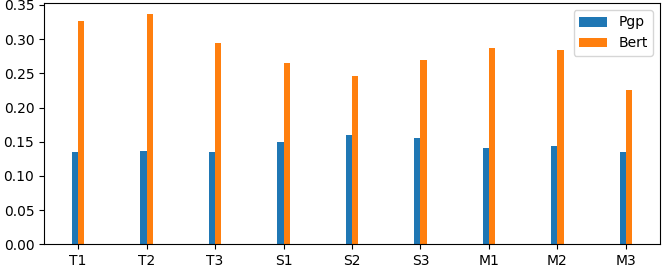
\includegraphics[width=\textwidth]{immagini/cpp}
\caption{Errori Corretti su errori presenti}
\end{figure}

\begin{figure}[H]
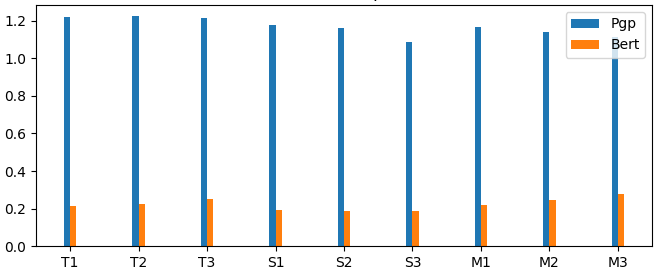
\includegraphics[width=\textwidth]{immagini/ips}
\caption{Errori introdotti per frase}
\end{figure}

\begin{figure}[H]
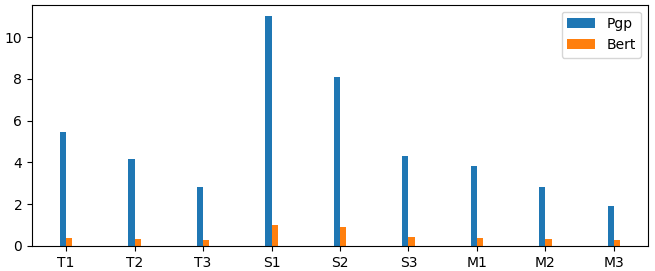
\includegraphics[width=\textwidth]{immagini/ipc}
\caption{Errori generati per errore corretto}
\end{figure}

I risultati mostrano come il correttore sviluppato presenti buone prestazioni, sopratutto nelle pipeline con solo errori di tokenizzazione.\\
\E\ particolarmente basso il numero di errori introdotti dal processo di correzione. Questo risultato è dovuto al modo in cui il sistema genera i candidati per la correzione. Essi infatti sono generati a partire dal contesto della frase e senza conoscere la parola da correggere. Ciò comporta che è possibile usare la distanza di Levenshtein per discriminare le varie possibilità, e lasciare la frase inalterata in caso, ad esempio, di falsi positivi.

\subsection{Considerazioni e Osservazioni}
Seguono alcune considerazioni sul sistema di correzione:
\begin{itemize}
\item La complessità di un'architettura come BERT comporta che il sistema sia abbastanza lento. Sicuramente utilizzare una macchina con dei CUDA cores darebbe uno speedup notevole, ma in ogni in caso il sistema è decisamente più lento di Pgp. Per queste ragioni, tutti i test sono stati eseguiti su una versione ridotta del dataset, composta da 10000 frasi scelte casualmente.
\item Il sistema potrebbe essere ulteriormente esteso per migliorarne le performance, specialmente per gli errori di segmentazione. Al momento, infatti non è stato possibile trovare un metodo efficace per la correzione dei segni di punteggiatura errati.
\item Nel dataset preso in considerazione, tutte le frasi hanno una lunghezza inferiore ai 50 caratteri. \E\ lecito pensare, dato il funzionamento del sistema di correzione, che ad una maggior lunghezza corrispondano risultati migliori.
\end{itemize}


\bibliographystyle{unsrt}
\bibliography{../bibliografia}














\end{document}